\documentclass[12pt,letterpaper, onecolumn]{exam}
\usepackage{amsmath}
\usepackage{amssymb}
\usepackage{commath}
\usepackage{physics}
\usepackage{multirow}
\usepackage{float}
\usepackage{relsize}
\usepackage{tikz}
\usepackage[lmargin=71pt, tmargin=1.2in]{geometry}  %For centering solution box
\usepackage{clrscode}
\usepackage{listings}
\usepackage{xcolor}
\usepackage{pdfpages}
\definecolor{codegreen}{rgb}{0,0.6,0}
\definecolor{codegray}{rgb}{0.5,0.5,0.5}
\definecolor{codepurple}{rgb}{0.58,0,0.82}
\definecolor{backcolour}{rgb}{0.95,0.95,0.92}
\usetikzlibrary{arrows.meta}
\usetikzlibrary{patterns}
\graphicspath{ {./images/} }

\lstdefinestyle{mystyle}{
    backgroundcolor=\color{backcolour},   
    commentstyle=\color{codegreen},
    keywordstyle=\color{magenta},
    numberstyle=\tiny\color{codegray},
    stringstyle=\color{codepurple},
    basicstyle=\ttfamily\footnotesize,
    breakatwhitespace=false,         
    breaklines=true,                 
    captionpos=b,                    
    keepspaces=true,                 
    numbers=left,                    
    numbersep=1pt,                  
    showspaces=false,                
    showstringspaces=false,
    showtabs=false,                  
    tabsize=2
}

%\lstset{style=mystyle}
\lhead{CAP 5610 Assignment \#1 Solution\\}
\rhead{Arman Sayan\\}
% \chead{\hline} % Un-comment to draw line below header
\thispagestyle{empty}   %For removing header/footer from page 1

\begin{document}

\begingroup  
    \centering
    \LARGE CAP 5610\\
    \LARGE Assignment \#1 Solution\\[0.5em]
    \large \today\\[0.5em]
    \large Arman Sayan\par
\endgroup
\rule{\textwidth}{0.4pt}
\bracketedpoints   %Self-explanatory
\printanswers
\renewcommand{\solutiontitle}{\noindent\textbf{Ans:}\enspace}   %Replace "Ans:" with starting keyword in solution box
\qformat{\large \textbf{\thequestion \quad \thequestiontitle \quad [\thepoints] \hfill}}
\renewcommand{\thepartno}{\arabic{partno}}
\renewcommand{\partlabel}{\thepartno.}

\begin{questions}
    \titledquestion{Decision Tree Basics}[30]
    
    %The goal of this assignment is to test and reinforce your understanding of Decision Tree Classifiers.
    
    \begin{parts}
      \part[5] Solution for Part 1:
      %How many unique, perfect binary trees of depth 3 can be drawn if we have 5 attributes? By depth, we mean the depth of the splits, not including the nodes that only contain a label (see Figure 1). So, a tree that checks just one attribute is a depth one tree. By perfect binary tree, we mean every node has either 0 or 2 children, and every leaf is at the same depth. Note also that a tree with the same attributes but organized at different depths is considered “unique”. Do not include trees that test the same attribute along the same path in the tree.

        %\begin{figure}[h]
        %    \centering
        %    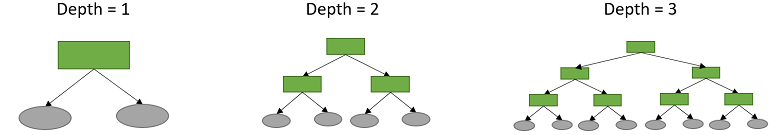
\includegraphics[width=\textwidth]{decision-tree-depth.png}
        %    \caption{Example of perfect binary trees with different depths.}
        %\end{figure}
      
      \begin{solution}

        Based on these definitions, to calculate the number of unique, perfect binary trees of depth 3 with 5 attributes,
        we need to clear out some key facts about this tree.

        First of all, since the depth of the tree is 3,
        This means the tree has 7 internal nodes, namely 1 root, 2 children, and 4 grandchildren, 
        and every path from the root to a leaf is of length 3.

        Secondly, since this tree has the perfect binary tree structure, every internal node should split into exactly two children,
        and every leaf should be at the same depth.

        Now that we clearly understand the structure of the tree, we can calculate the number of unique trees.

        The first step is to choose 3 attributes for a path. There are 5 attributes which can be (A,B,C,D,E),
        and for any given path, we need to select 3 distinct attributes. The number of ways to do this is

        \begin{center}
            $\displaystyle{\binom{5}{3} = \frac{5!}{3!(5-3)!} = 10}$
        \end{center}

        So, there are 10 ways to choose which 3 attributes will appear along a given path.

        The second step is to choose the order of the attributes along the path.
        Once we have selected 3 attributes for a path, we can arrange them in $3!$ ways
        since the order of the attributes matters.

        \begin{center}
            $\displaystyle{3! = 6}$
        \end{center}

        So, for each choice of attributes, there are $6$ unique ways to organize them along a path.

        Since the tree is a perfect binary tree, all paths must have the same set of attributes arranged in the same way.

        Thus, we only count how many ways we can assign attributes to the tree consistently, which is 

        \begin{center}
            Number of ways to choose 3 attributes $\displaystyle{\cross}$ Number of ways to arrange them in depth order

            $\boldsymbol{\displaystyle{\binom{5}{3} \cdot 3! = 10 \cdot 6 = 60}}$
        \end{center}

        Therefore, there are $\boldsymbol{60}$ unique, perfect binary trees of depth 3 with 5 attributes.

      \end{solution}

      \pagebreak
      
      \part[5] Solution for Part 2:
      %In general, for a problem with $A$ attributes, how many unique perfect $D$ depth trees can be drawn? Assume $A >> D$.

      \begin{solution}

        To calculate the number of unique perfect binary trees of depth 
        $D$ with $A$ attributes $A >> D$, we need to generalize the reasoning we used in earlier question.

        The first step is to choose $D$ attributes from the $A$ available attributes.
        The number of ways to do this is actually

        \begin{center}
            $\displaystyle{\binom{A}{D} = \frac{A!}{D!(A-D)!}}$
        \end{center}

        The second step is Once the $D$ attributes are chosen,
        we must arrange them in a specific order to determine their position in the tree, which might be root, children, grandchildren, etc.,
        the number of ways to arrange $D$ attributes is

        \begin{center}
            $\displaystyle{D!}$
        \end{center}

        The last step is to combine these values to calculate the total number of unique trees.
        The general formula for total number of unique perfect binary trees of depth $D$ with $A$ attributes is

        \begin{center}
            \textbf{Total Trees} $\boldsymbol{\displaystyle{ = \binom{A}{D} \cdot D! = \frac{A!}{D!(A-D)!} \cdot D! = \frac{A!}{(A-D)!}}}$
        \end{center}

      \end{solution}

      \pagebreak
      
      \part[10] Solution for Part 3:
      %Consider the following dataset from Table 1 for this problem. Given the five attributes on the left, we want to predict if the student got an A in the course. Create 2 decision trees for this dataset. For the first, only go to depth 1. For the second go to depth 2. For all trees, use the ID3 entropy algorithm from class. For each node of the tree, show the decision, the number of positive and negative examples and show the entropy at that node.

      %Hint: There are a lot of calculations here. You may want to do this programatically.

        %\begin{table}[!h]
        %    \begin{center}
        %    \begin{tabular}{c | c | c | c| c || c}
        %        \hline
        %        Early & Finished HMK & Senior & Likes Coffee & Liked The Last Jedi & A \\
        %        \hline
        %        \hline
        %        1 & 1 & 0 & 0 & 1 & 1 \\
        %        \hline
        %        1 & 1 & 1 & 0 & 1 & 1 \\
        %        \hline
        %        0 & 0 & 1 & 0 & 0 & 0 \\
        %        \hline
        %        0 & 1 & 1 & 0 & 1 & 0 \\ 
        %        \hline
        %        0 & 1 & 1 & 0 & 0 & 1 \\
        %        \hline
        %        0 & 0 & 1 & 1 & 1 & 1 \\ 
        %        \hline
        %        1 & 0 & 0 & 0 & 1 & 0 \\
        %        \hline
        %        0 & 1 & 0 & 1 & 1 & 1 \\ 
        %        \hline
        %        0 & 0 & 1 & 0 & 1 & 1 \\
        %        \hline
        %        1 & 0 & 0 & 0 & 0 & 0 \\ 
        %        \hline
        %        1 & 1 & 1 & 0 & 0 & 1 \\
        %        \hline
        %        0 & 1 & 1 & 1 & 1 & 0 \\ 
        %        \hline
        %        0 & 0 & 0 & 0 & 1 & 0 \\
        %        \hline
        %        1 & 0 & 0 & 1 & 0 & 1 \\ 
        %        \hline
        %    \end{tabular}
        %    \end{center}
        %    \caption{Toy Data-set for Task 1: Decision Tree Basics.}
        %\end{table}
      
      \begin{solution}

        To create two decision trees (depth 1 and depth 2) using the ID3 entropy
        algorithm, we need to calculate the entropy for the root node and each split, 
        and then select the attribute that minimizes the weighted average entropy, 
        namely maximizes information gain at each step, and split the dataset accordingly.

        The first step is to calculate the entropy for the root node.

        \begin{center}
            $\displaystyle{H(S) = -p_1 \log_2 p_1 - p_0 \log_2 p_0}$
        \end{center}

        where $p_1$ is the probability of $(A=1)$ 
        and $p_0$ is the probability of $(A=0)$.

        The second step is for each attribute, we need to calculate the 
        weighted average entropy of splitting on that attribute as below

        \begin{center}
            $\displaystyle{H_{split} = \sum_{v \in Values} \frac{|S_v|}{|S|} H(S_v)}$
        \end{center}

        where $S_v$ is the subset of the dataset where the attribute takes 
        the value $v$, and $H(S_v)$ is its entropy.

        The third step is to calculate the information gain for each attribute, which is

        \begin{center}
            $\displaystyle{IG = H(S) - H_{split}}$
        \end{center}

        The attribute with the highest information gain is selected as the attribute to be splitted.

        The last step is to repeat this process for each subset until the tree reaches the desired depth.

        The Python implementation of this algorithm is included in the appendix named as
    
        \begin{center}
            \textbf{CAP\_5610\_Assignment\_1\_Solution\_Arman\_Sayan.ipynb}
        \end{center}

        The decision trees for depth 1 and depth 2 computed by this Python code 
        are visualized in the following figures:
        
        \begin{figure}[H]
            \begin{center}
                \begin{minipage}{0.85\textwidth}
                        \centering
                        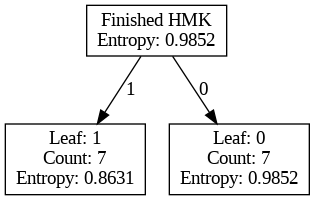
\includegraphics[width=0.8\textwidth]{depth_1_tree.png}
                        \caption{Decision Tree with Depth 1}
                \end{minipage}
            \end{center}
        \end{figure}
        

        \begin{figure}[H]
            \begin{minipage}{\textwidth} 
                \centering
                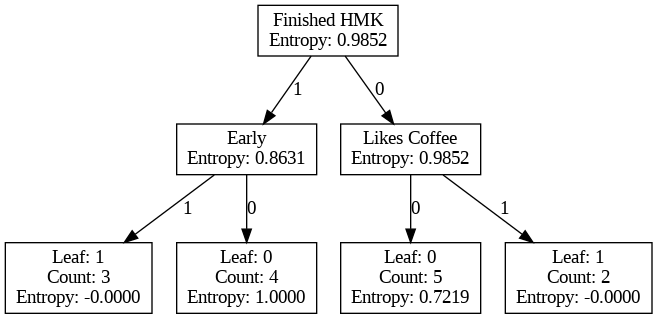
\includegraphics[width=\textwidth]{depth_2_tree.png}
                \caption{Decision Tree with Depth 2}
            \end{minipage}
        \end{figure}

      \end{solution}

      \pagebreak

      \part[5] Solution for Part 4:
      %Make one more decision tree. Use the same procedure as in (3), but make it depth 3. Now, given these three trees, which would you prefer if you wanted to predict the grades of 10 new students who are not included in this data-set? Justify your choice.

      \begin{solution}

        The decision tree for depth 3 computed by the same Python code used in (3)
        is visualized in the following figure:

        \begin{figure}[H]
            \begin{minipage}{\textwidth} 
                \centering
                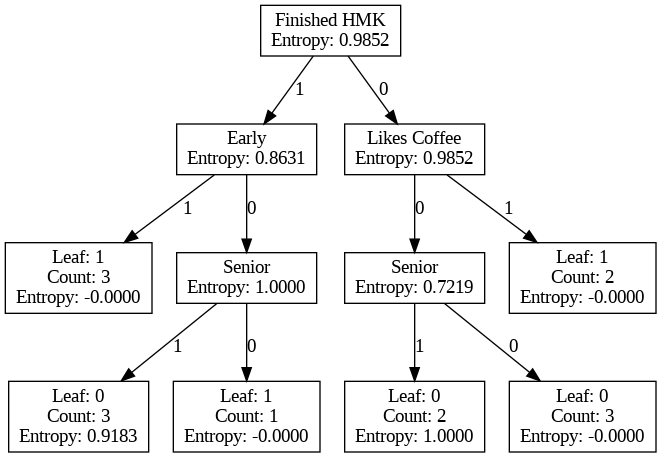
\includegraphics[width=\textwidth]{depth_3_tree.png}
                \caption{Decision Tree with Depth 3}
            \end{minipage}
        \end{figure}

        Given these three trees, if we wanted to predict the grades of 10 new students who are not included in this data-set,

        I would prefer the decision tree with depth 2. The reason for this choice is that the decision tree with depth 2 is the overall model among the three trees.

        The decision tree with depth 1 is too simple and may not capture the underlying patterns in the data,
        while the decision tree with depth 3 is too complex and may overfit the training data.

        The decision tree with depth 2 strikes a good balance between simplicity and complexity,
        making it more likely to generalize well to new, unseen data.

        Furthermore, we can also compare the average entropy of the leaf nodes for each tree.
        A lower average entropy at the leaves implies a more confident prediction at each leaf.
        This would make it preferable if accuracy is the primary goal.

        Based on these calculated decision trees, the average entropy of the leaf nodes for each tree is as follows:
        
        \begin{itemize}
            \item Depth 1 Tree: 0.9242
            \item Depth 2 Tree: 0.4305
            \item Depth 3 Tree: 0.3197
        \end{itemize}

        We can see that the average entropy of the leaf nodes decreases as the depth of the tree increases.
        This implies that the decision tree with depth 3 is more confident in its predictions compared to the other trees.
        However, there is not significant difference between depth 2 value and depth 3 value and
        there is still the chance that a decision tree with depth 3 might overfit the data, 
        making it less generalizable to new students.

      
      \end{solution}

      \pagebreak

      \part[5] Solution for Part 5:
      %Consider a new definition of a “realizable” case: “For some fixed concept class $C$, such as decision trees, a realizable case is one where the algorithm gets a sample consistent with some concept $c \in C$. In other words, for decision trees, a case is realizable if there is some tree that perfectly classifies the data-set.
    
      %If the number of attributes $A$ is sufficiently large, under what condition would a dataset not 
      %be realizable for decision trees of no fixed depth? Prove that the dataset is unrealizable if 
      %and only if that condition is true.

      \begin{solution}

        For a dataset to not be realizable for decision trees of depth $n$,
        there should be at least one combination of input attributes and labels 
        in the dataset that cannot be represented or separated by a decision tree 
        of depth $n$, regardless of the size of the attribute space $A$.

        For instance, a decision tree of depth $n$ can split the data into at most $2^n$
        leaf nodes, and each leaf node corresponds to one subset of the input space uniquely.

        So, if the dataset has more unique combinations of input features that 
        need to be classified differently than can be represented by $2^n$ leaf nodes,
        then the dataset cannot be realizable for a decision tree of depth $n$.

        Formally, for a dataset with $m$ distinct examples, a depth with $n$
        decision tree can perfectly classify the dataset only if $m \leq 2^n$.

        It is also important to note that the size of the attribute space $A$ does 
        not affect the realizability of the dataset. A larger $A$ provides more potential 
        splits for the tree. However, the depth of the tree, not the attribute count, 
        determines the maximum number of partitions $2^n$ that the tree can form.

        Therefore, \textbf{if $\boldsymbol{m > 2^n}$, the dataset is not realizable for decision trees of $\boldsymbol{n}$,
        regardless of the size of the attribute space $\boldsymbol{A}$}.
      
      \end{solution}
      
    \end{parts}

    \pagebreak

    \titledquestion{Application of Decision Tree on Real-Word Data-set}[25]

    \begin{parts}

        \part[10] Solution for Part 1:
        %Train a decision tree classifier using the data file. Vary the cut-off depth from 2 to 10 and report the training accuracy for each cut-off depth $k$. Based on your results, select an optimal $k$.

        \begin{solution}

            Please check the source code and outputs included in the appendix named as
    
            \begin{center}
                \textbf{CAP\_5610\_Assignment\_1\_Solution\_Arman\_Sayan.ipynb}
            \end{center}
            
            for the solution.
        \end{solution}

        \part[8] Solution for Part 2:
        %Using the trained classifier with optimal cut-off depth $k$, classify the 99,762 instances from the test file and report the testing accuracy (the portion of testing instances classified correctly).

        \begin{solution}

            Please check the source code and outputs included in the appendix named as
    
            \begin{center}
                \textbf{CAP\_5610\_Assignment\_1\_Solution\_Arman\_Sayan.ipynb}
            \end{center}
            
            for the solution.
        \end{solution}

        \part[7] Solution for Part 3:
        %Do you see any over-fitting issues for this experiment? Report your observations.

        \begin{solution}

            Please check the source code and outputs included in the appendix named as
    
            \begin{center}
                \textbf{CAP\_5610\_Assignment\_1\_Solution\_Arman\_Sayan.ipynb}
            \end{center}
            
            for the solution.
        \end{solution}
        
    \end{parts}

    \pagebreak

    \titledquestion{Independent Events and Bayes Theorem}[20]

    \begin{parts}

        \part[5] Solution for Part 1:
        %For events $A$, $B$ prove:

        %\begin{center}
        %    $\displaystyle{P(A|B) = \frac{P(B|A)P(A)}{P(B|A)P(A) + P(B|\lnot A)P(\lnot A)}}$
        %\end{center}

        %($\lnot A$ denotes the event that $A$ does not occur.)

        \begin{solution}

            We need to prove Bayes' theorem in the expanded form. We know from Bayes' rule that the definition of conditional probability is
            
            \begin{center}
                $\displaystyle{P(A|B) = \frac{P(A \cap B)}{P(B)}}$
            \end{center}

            By a simple induction, we can write $\displaystyle{P(A \cap B)}$ as

            \begin{center}
                $\displaystyle{P(A \cap B)= P(B|A)P(A)}$
            \end{center}

            Furthermore, using the law of total probability, we can express $\displaystyle{P(B)}$ as

            \begin{center}
                $\displaystyle{P(B) = P(A \cap B) + P(\lnot A \cap B)}$
            \end{center}

            where by using the above induction again, we reveal that

            \begin{center}
                $\displaystyle{P(\lnot A \cap B)= P(B|\lnot A)P(\lnot A)}$
            \end{center}

            Using these definitions and substituting them in the original theorem, we can prove that 

            \begin{center}
                $\boldsymbol{\displaystyle{P(A|B) = \frac{P(A \cap B)}{P(B)}}}$

                $\boldsymbol{\displaystyle{P(A|B) = \frac{P(B|A)P(A)}{P(A \cap B) + P(\lnot A \cap B)}}}$

                $\boldsymbol{\displaystyle{P(A|B) = \frac{P(B|A)P(A)}{P(B|A)P(A) + P(B|\lnot A)P(\lnot A)}}}$
            \end{center}

        \end{solution}

        \pagebreak

        \part
        %Let $X$, $Y$ , and $Z$ be random variables taking values in ${0, 1}$. The following table lists the probability of each possible assignment of 0 and 1 to the variables $X$, $Y$, and $Z$:

        %                  \begin{table}[!h]
        %    \begin{center}
        %    \begin{tabular}{c | c | c | c | c}
        %        \hline
        %        \multirow{2}{4em}{} & \multicolumn{2}{c|}{ \textbf{$Z=0$}  } & \multicolumn{2}{c}{ \textbf{$Z=1$}  }\\ 
        %        \hline
        %        \textbf{} & $X=0$ & $X=1$ & $X=0$ & $X=1$ \\ 
        %        %\multicolumn{4}{c|}{ y } \\
        %        %&  & y & \\
        %        \hline
        %        $Y=0$ & 0.1 & 0.05 & 0.1 & 0.1 \\ 
        %        \hline
        %        $Y=1$ & 0.2 & 0.1 & 0.175 & 0.175 \\ 
        %        \hline
        %    \end{tabular}
        %    \end{center}
        %    \end{table}

        \begin{subparts}

            \subpart[5] Solution for Part 2.i:
            %Is $X$ independent of $Y$? Why or why not?
    
            \begin{solution}

                To determine if $X$ and $Y$ are independent, we need to check whether the joint probability
                $P(X=x,Y=y)$ equals the product of the marginal probabilities 
                $P(X=x) \cdot P(Y=y)$ for all possible values of $x$ and $y$. If this holds true for all combinations, 
                $X$ and $Y$ are independent. Otherwise, they are dependent.

                As the first step, we need to calculate the marginal probabilities.
                The formula for marginal probability $P(X=x,Y=y)$ is given as

                \begin{center}
                    $\displaystyle{P(X=x,Y=y) = P(X=x,Y=y,Z=0) + P(X=x,Y=y,Z=1)}$
                \end{center}

                For each combination of $X$ and $Y$, we can calculate the marginal probabilities as follows:

                \begin{itemize}
                    \item $P(X=0,Y=0) = P(X=0,Y=0,Z=0) + P(X=0,Y=0,Z=1) = 0.1 + 0.1 = 0.2$
                    \item $P(X=1,Y=0) = P(X=1,Y=0,Z=0) + P(X=1,Y=0,Z=1) = 0.05 + 0.1 = 0.15$
                    \item $P(X=0,Y=1) = P(X=0,Y=1,Z=0) + P(X=0,Y=1,Z=1) = 0.2 + 0.175 = 0.375$
                    \item $P(X=1,Y=1) = P(X=1,Y=1,Z=0) + P(X=1,Y=1,Z=1) = 0.1 + 0.175 = 0.275$
                \end{itemize}

                Now, we can calculate the marginal probabilities $P(X)$ and $P(Y)$ as follows:

                \begin{itemize}
                    \item $P(X=0) = P(X=0,Y=0) + P(X=0,Y=1) = 0.2 + 0.375 = 0.575$
                    \item $P(X=1) = P(X=1,Y=0) + P(X=1,Y=1) = 0.15 + 0.275 = 0.425$
                    \item $P(Y=0) = P(X=0,Y=0) + P(X=1,Y=0) = 0.2 + 0.15 = 0.35$
                    \item $P(Y=1) = P(X=0,Y=1) + P(X=1,Y=1) = 0.375 + 0.275 = 0.65$
                \end{itemize}

                The second step is to check the independce, which means for $X$ and $Y$ to be independent, the following must hold:

                \begin{center}
                    $\displaystyle{P(X=x,Y=y) = P(X=x) \cdot P(Y=y)}$
                \end{center}
                
                Check $P(X=0,Y=0)$:

                \begin{center}
                    $P(X=0,Y=0) = 0.2$

                    $P(X=0) \cdot P(Y=0) = 0.575 \cdot 0.35 = 0.20125$

                    $\boldsymbol{P(X=0,Y=0) \neq P(X=0) \cdot P(Y=0)}$
                \end{center}

                Check $P(X=1,Y=0)$:

                \begin{center}
                    $P(X=1,Y=0) = 0.15$

                    $P(X=1) \cdot P(Y=0) = 0.425 \cdot 0.35 = 0.14875$

                    $\boldsymbol{P(X=1,Y=0) \neq P(X=1) \cdot P(Y=0)}$
                \end{center}

                Check $P(X=0,Y=1)$:

                \begin{center}
                    $P(X=0,Y=1) = 0.375$

                    $P(X=0) \cdot P(Y=1) = 0.575 \cdot 0.65 = 0.37375$

                    $\boldsymbol{P(X=0,Y=1) \neq P(X=0) \cdot P(Y=1)}$
                \end{center}

                Check $P(X=1,Y=1)$:

                \begin{center}
                    $P(X=1,Y=1) = 0.275$

                    $P(X=1) \cdot P(Y=1) = 0.425 \cdot 0.65 = 0.27625$

                    $\boldsymbol{P(X=1,Y=1) \neq P(X=1) \cdot P(Y=1)}$
                \end{center}

                The values $P(X=x,Y=y)$ and $P(X=x)P(Y=y)$ are not exactly equal for all combinations. 
                Therefore, \textbf{$\boldsymbol{X}$ and $\textbf{Y}$ are not independent}.
                
            \end{solution}

            \pagebreak

            \subpart[5] Solution for Part 2.ii:
            %Is $X$ conditionally independent of $Y$ given $Z$? Why or why not?
    
            \begin{solution}

                To determine whether $X$ is conditionally independent of $Y$ given 
                $Z$, we need to verify if the following holds for all values of 
                $X$, $Y$, and $Z$:
                
                \begin{center}
                    $\displaystyle{P(X|Y,Z) = P(X|Z)}$
                \end{center}

                The formula for conditional probability $P(X|Y,Z)$ is given as

                \begin{center}
                    $\displaystyle{P(X|Y,Z) = \frac{P(X,Y,Z)}{P(Y,Z)}}$
                \end{center}

                The first step is to calculate the joint probabilities $P(X,Y,Z)$ for all combinations of $X$, $Y$, and $Z$.
                We can use the values from the table as it is.

                The second step is to calculate the marginal probabilities $P(Y,Z)$ for all combinations of $Y$ and $Z$.

                \begin{itemize}
                    \item $P(Y=0,Z=0) = P(X=0,Y=0,Z=0) + P(X=1,Y=0,Z=0) = 0.1 + 0.05 = 0.15$
                    \item $P(Y=1,Z=0) = P(X=0,Y=1,Z=0) + P(X=1,Y=1,Z=0) = 0.2 + 0.1 = 0.3$
                    \item $P(Y=0,Z=1) = P(X=0,Y=0,Z=1) + P(X=1,Y=0,Z=1) = 0.1 + 0.1 = 0.2$
                    \item $P(Y=1,Z=1) = P(X=0,Y=1,Z=1) + P(X=1,Y=1,Z=1) = 0.175 + 0.175 = 0.35$
                \end{itemize}

                The third step is to calculate the conditional probabilities $P(X|Y,Z)$ and $P(X|Z)$. We will have 2 cases to check.

                The first case is when $Z=0$:

                First, we compute the probabilities $P(Y, Z=0)$ which are obtained by summing over all $X$:

                \begin{itemize}
                    \item $P(Y=0, Z=0) = P(X=0, Y=0, Z=0) + P(X=1, Y=0, Z=0) = 0.1 + 0.05 = 0.15$
                    \item $P(Y=1, Z=0) = P(X=0, Y=1, Z=0) + P(X=1, Y=1, Z=0) = 0.2 + 0.1 = 0.3$
                    
                    \begin{center}
                        $P(Z=0) = P(Y=0, Z=0) + P(Y=1, Z=0) = 0.15 + 0.3 = 0.45$
                    \end{center}
                \end{itemize}

                Second, we compute the probabilities $P(X, Z=0)$ which are obtained by summing over all $Y$:

                \begin{itemize}
                    \item $P(X=0, Z=0) = P(X=0, Y=0, Z=0) + P(X=0, Y=1, Z=0) = 0.1 + 0.2 = 0.3$
                    \item $P(X=1, Z=0) = P(X=1, Y=0, Z=0) + P(X=1, Y=1, Z=0) = 0.05 + 0.1 = 0.15$
                \end{itemize}

                Third, we compute the probability $P(X|Z=0)$:

                \begin{itemize}
                    \item $\displaystyle{P(X=0|Z=0) = \frac{P(X=0, Z=0)}{P(Z=0)} = \frac{0.3}{0.45} = 0.666}$
                    \item $\displaystyle{P(X=1|Z=0) = \frac{P(X=1, Z=0)}{P(Z=0)} = \frac{0.15}{0.45} = 0.333}$
                \end{itemize}

                Fourth, we compute the probability $P(X|Y, Z=0)$:

                \begin{itemize}
                    \item For $Y=0$:
                    \begin{center}
                    $\displaystyle{P(X=0|Y=0, Z=0) = \frac{P(X=0, Y=0, Z=0)}{P(Y=0, Z=0)} = \frac{0.1}{0.15} = 0.666}$

                    $\displaystyle{P(X=1|Y=0, Z=0) = \frac{P(X=1, Y=0, Z=0)}{P(Y=0, Z=0)} = \frac{0.05}{0.15} = 0.333}$
                    \end{center}

                    \item For $Y=1$:
                    \begin{center}
                    $\displaystyle{P(X=0|Y=1, Z=0) = \frac{P(X=0, Y=1, Z=0)}{P(Y=1, Z=0)} = \frac{0.2}{0.3} = 0.666}$

                    $\displaystyle{P(X=1|Y=1, Z=0) = \frac{P(X=1, Y=1, Z=0)}{P(Y=1, Z=0)} = \frac{0.1}{0.3} = 0.333}$
                    \end{center}
                \end{itemize}

                Since $P(X|Y, Z=0) = P(X|Z=0)$ for all values of $X$, the condition holds for $Z=0$.

                The second case is when $Z=1$:

                First, we compute the probabilities $P(Y, Z=1)$ which are obtained by summing over all $X$:

                \begin{itemize}
                    \item $P(Y=0, Z=1) = P(X=0, Y=0, Z=1) + P(X=1, Y=0, Z=1) = 0.1 + 0.1 = 0.2$
                    \item $P(Y=1, Z=1) = P(X=0, Y=1, Z=1) + P(X=1, Y=1, Z=1) = 0.175 + 0.175 = 0.35$
                    
                    \begin{center}
                        $P(Z=1) = P(Y=0, Z=1) + P(Y=1, Z=1) = 0.2 + 0.35 = 0.55$
                    \end{center}
                \end{itemize}

                Second, we compute the probabilities $P(X, Z=1)$ which are obtained by summing over all $Y$:

                \begin{itemize}
                    \item $P(X=0, Z=1) = P(X=0, Y=0, Z=1) + P(X=0, Y=1, Z=1) = 0.1 + 0.175 = 0.275$
                    \item $P(X=1, Z=1) = P(X=1, Y=0, Z=1) + P(X=1, Y=1, Z=1) = 0.1 + 0.175 = 0.275$
                \end{itemize}

                Third, we compute the probability $P(X|Z=1)$:

                \begin{itemize}
                    \item $\displaystyle{P(X=0|Z=1) = \frac{P(X=0, Z=1)}{P(Z=1)} = \frac{0.275}{0.55} = 0.5}$
                    \item $\displaystyle{P(X=1|Z=1) = \frac{P(X=1, Z=1)}{P(Z=1)} = \frac{0.275}{0.55} = 0.5}$
                \end{itemize}

                Fourth, we compute the probability $P(X|Y, Z=1)$:

                \begin{itemize}
                    \item For $Y=0$:
                    \begin{center}
                    $\displaystyle{P(X=0|Y=0, Z=1) = \frac{P(X=0, Y=0, Z=1)}{P(Y=0, Z=1)} = \frac{0.1}{0.2} = 0.5}$

                    $\displaystyle{P(X=1|Y=0, Z=1) = \frac{P(X=1, Y=0, Z=1)}{P(Y=0, Z=1)} = \frac{0.1}{0.2} = 0.5}$
                    \end{center}

                    \item For $Y=1$:
                    \begin{center}
                    $\displaystyle{P(X=0|Y=1, Z=1) = \frac{P(X=0, Y=1, Z=1)}{P(Y=1, Z=1)} = \frac{0.175}{0.35} = 0.5}$

                    $\displaystyle{P(X=1|Y=1, Z=1) = \frac{P(X=1, Y=1, Z=1)}{P(Y=1, Z=1)} = \frac{0.175}{0.35} = 0.5}$
                    \end{center}
                \end{itemize}

                Like in the first case, Since $P(X|Y, Z=1) = P(X|Z=1)$ for all values of $X$, the condition holds for $Z=1$.

                For all values of $Z$, we proved that 

                \begin{center}
                    $\displaystyle{P(X|Y,Z) = P(X|Z)}$
                \end{center}

                Thus, \textbf{X is conditionally independent of Y given Z}.

            \end{solution}

            \pagebreak

            \subpart[5] Solution for Part 2.iii:
            %Calculate $P (X \neq Y |Z = 0)$.
    
            \begin{solution}

                To compute $P(X \neq Y | Z = 0)$, we need to calculate the probability of events where $X \neq Y$, 
                such as $X=0$ and $Y=1$, or $X=1$ and $Y=0$, conditioned on $Z = 0$.

                We can calculate the probability as follows:

                \begin{center}
                    $\displaystyle{P(X \neq Y | Z = 0) = \frac{P(X \neq Y, Z = 0)}{P(Z=0)}}$
                \end{center}

                Furthermore, we can calculate $P(X \neq Y, Z = 0)$ as

                \begin{center}
                    $\displaystyle{P(X \neq Y, Z = 0) = P(X=0, Y=1, Z=0) + P(X=1, Y=0, Z=0)}$
                \end{center}

                From the table, we can find the values as

                \begin{itemize}
                    \item $P(X=0, Y=1, Z=0) = 0.2$
                    \item $P(X=1, Y=0, Z=0) = 0.05$
                    
                \begin{center}
                    $\displaystyle{P(X \neq Y, Z = 0) = 0.2 + 0.05 = 0.25}$
                \end{center}
                \end{itemize}

                In addition, we need to calculate $P(Z=0)$ by summing all joint probabilities where $Z=0$:

                \begin{center}
                    $\displaystyle{P(Z=0) = P(X=0, Y=0, Z=0) + P(X=1, Y=0, Z=0)}$

                    $\displaystyle{+ P(X=0, Y=1, Z=0) + P(X=1, Y=1, Z=0)}$

                    $\displaystyle{= 0.1 + 0.05 + 0.2 + 0.1 = 0.45}$
                \end{center}

                Finally, by substituting the values, we can calculate $P(X \neq Y | Z = 0)$ as

                \begin{center}
                    $\boldsymbol{\displaystyle{P(X \neq Y | Z = 0) = \frac{0.25}{0.45} \approx 0.5556}}$
                \end{center}
                
                
            \end{solution}
            
        \end{subparts}
  
    \end{parts}

    \pagebreak

    \titledquestion{Implementing Naive Bayes}[25]

    %You will now learn how to use Naive Bayes Algorithm to solve a real-world problem: text cat-
    %egorization. Text categorization (also referred to as text classification) i s t he t ask o f assigning
    %documents to one or more topics. For our homework, we will use a benchmark dataset that is fre-
    %quently used in text categorization problems. This dataset, Reuters-21578, consists of documents that
    %appeared in Reuters newswire in 1987. Each document was then manually categorized into a topic
    %among over 100 topics. In this homework, we are only interested in earn and acquisition (acq) topics,
    %so we will use a shortened version of the dataset (documents assigned to topics other than “earn” or
    %“acq” are not in the dataset provided for the homework). As features, we will use the frequency
    %(counts) of each word that occurred in the document. This model is known as the bag-of-words model
    %and it is frequently used in text categorization. You can download Assignment 2 data from the Canvas.
    %In this folder, you will find:
    %
    %\begin{itemize}
    %    \item \textbf{train.csv:} Training data. Each row represents a document, and each column separated by
    %    commas represents features (word counts). There are 4527 documents and 5180 words.
    %    \item \textbf{train labels.txt:} labels for the training data
    %    \item \textbf{test.csv:} Test data, 1806 documents and 5180 words
    %\end{itemize}
    %
    %Implement Naive Bayes Algorithm. Train your classifier on the training set that is given and report training accuracy, testing accuracy, and the amount of time spent training the classifier.

    Solution for Q4:

    \begin{solution}

        Please check the source code and outputs included in the appendix named as
    
        \begin{center}
            \textbf{CAP\_5610\_Assignment\_1\_Solution\_Arman\_Sayan.ipynb}
        \end{center}
            
        for the solution.
    \end{solution}

    \pagebreak
    
\end{questions}

\begin{appendix}
    \centering
    \begin{flushleft}  
      \section{Appendix}
      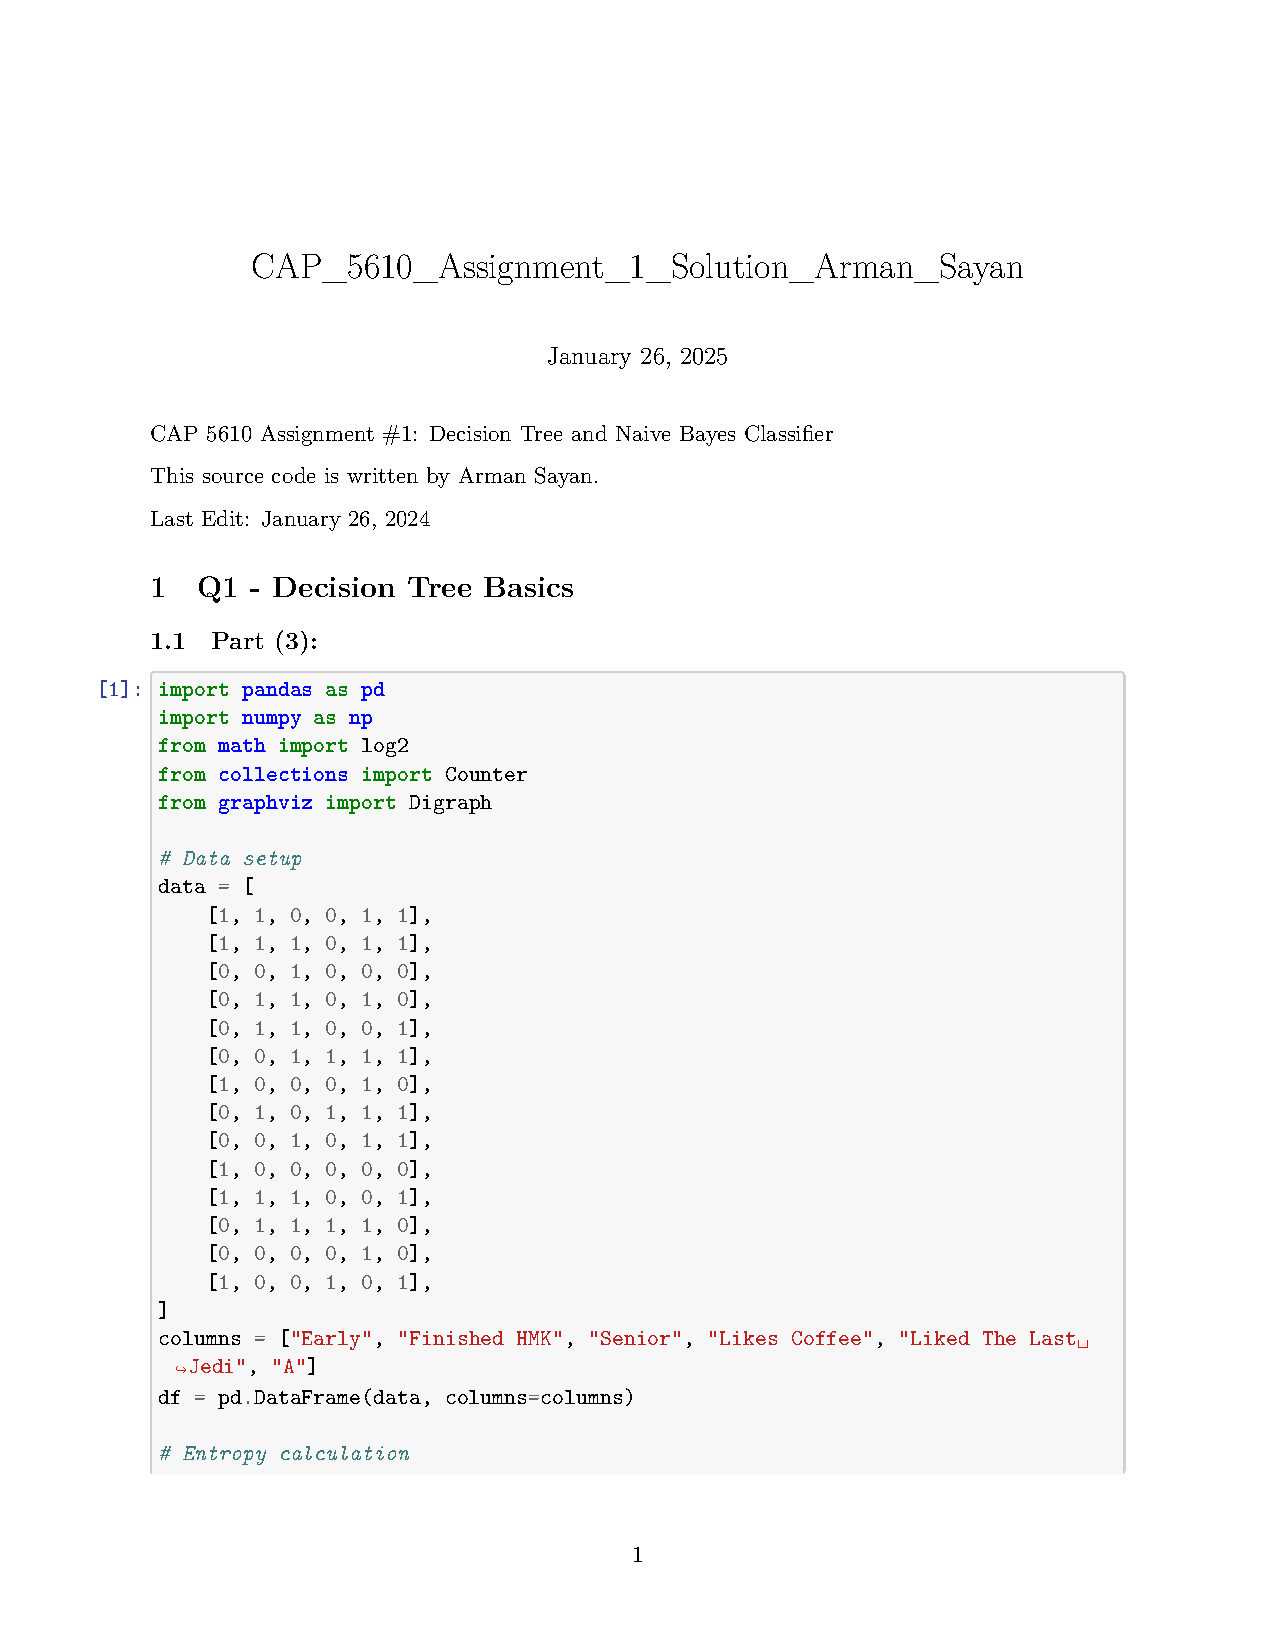
\includepdf[pages=-]{CAP_5610_Assignment_1_Solution_Arman_Sayan_1.pdf}
    \end{flushleft}
\end{appendix}

\end{document}